%\documentclass[a0,landscape,posterdraft]{a0poster}
%\documentclass[a0b,landscape,final]{a0poster}
\documentclass[a0b,portrait,final]{a0poster}
\usepackage{colordvi,amsmath,epsfig,float,color,multicol,subfigure}
%\usepackage{grffile}
\usepackage[table]{xcolor}
\usepackage{pstricks,pst-node}
%\usepackage{txfonts}
\usepackage{tabularx}
\usepackage[framemethod=TikZ]{mdframed}
\usepackage{lipsum}

% landscape
% portrait
% a0b   ``DIN A0 big''. 915.1* 1200 mm 
% a0    ``DIN A0''.    839.6 * 1188.2 mm
% draft                 Gj�r om til A4 for testutskrift.
% final                 Gj�r at PS-fila blir i spesifisert st�rrelse;
%                       standard.
% ISO A0 size, 841 mm by 1189 mm.
% \tiny            12pt
% \scriptsize      14.4pt
% \footnotesize    17.28pt
% \small           20.74pt
% \normalsize      24.88pt
% \large           29.86pt
% \Large           35.83pt
% \LARGE           43pt
% \huge            51.6pt
% \Huge            61.92pt
% \veryHuge        74.3pt
% \VeryHuge        89.16pt
% \VERYHuge        107pt

% N�r du har kj�rt latex 'filnavn.tex', vil det dukke opp en fil til i
% katalogen; 'a0header.ps'. Denne filen m� ligge der n�r du kj�rer
% dvips.

%%%%%%%%%%%%%
%  Lengder: %c
%%%%%%%%%%%%%

\addtolength{\textwidth}{-5cm}
\addtolength{\oddsidemargin}{0.2cm}

% Avstanden mellom kolonnene i multicolumn-mode
\setlength{\columnsep}{2.0cm}
\setlength{\parindent}{0cm}
\setlength{\parskip}{1.4ex}

%\pagestyle{empty}

% Setter standard skrifttype til � v�re 'phv'; Sans Serif.
\renewcommand{\familydefault}{phv}
% Setter standard skriftst�rrelse.
%renewcommand{\normalsize}{\huge}


\definecolor{DarkBlue}{rgb}{0.0470,0,0.5294}
\definecolor{rltred}{rgb}{0.75,0,0}
\definecolor{rltgreen}{rgb}{,0.0470,0.5294,0}
\definecolor{rltblue}{rgb}{0,0,0.75}
\definecolor{DarkRed}{rgb}{0.75, 0, 0.09}
\definecolor{ForestGreen}{rgb}{0, 0.27, 0.13}
\definecolor{NapierGreen}{rgb}{0.16, 0.5, 0.0}
\definecolor{NavyBlue}{rgb}{0.0, 0.0, 0.5}
% see http://en.wikipedi,a.org/wiki/List_of_colors for RGB 

\makeatletter

\renewcommand{\section}{\@startsection
        {section}%                          % the name 
        {1}%                                % the level
        {0mm}%                              % the indent
        {-\baselineskip}%                   % the beforeskip
        {1mm}%                              % the afterskip
        {\LARGE\color{DarkBlue}\bfseries}}% % the style

\renewcommand{\subsection}{\@startsection
        {subsection}%                       % the name 
        {2}%                                % the level
        {1mm}%                              % the indent
        {-0.9\baselineskip}%                % the beforeskip
        {1mm}%                              % the afterskip
        {\Large\color{DarkRed}\bfseries}}% % the style
\renewcommand{\subsubsection}{\@startsection
        {subsubsection}%                    % the name 
        {3}%                                % the level
        {4mm}%                              % the indent
        {-0.7\baselineskip}%                % the beforeskip
        {1mm}%                              % the afterskip
        {\large\color{ForestGreen}\bfseries}}% % the style
\renewcommand{\paragraph}{\@startsection
        {paragraph}%                        % the name 
        {4}%                                % the level
        {6mm}%                              % the indent
        {-0.9\baselineskip}%                % the beforeskip
        {0mm}%                              % the afterskip
        {\large\color{NavyBlue}\slshape}}% % the style
\makeatother

\begin{document}
\begin{minipage}[t]{0.8\linewidth}
  {\veryHuge \textbf{DESIGN AND DEVELOPMENT OF THE ECR ION SOURCE CONTROL SYSTEM}}
  \\[1ex]
  \bigskip
     {\LARGE Hyungjoo Son} {\large \texttt{hjson@ibs.re.kr}}, 
     {Sangil Lee} {\texttt{silee@ibs.re.kr}},
     {Chang Wook Son} {\texttt{scwook@ibs.re.kr}},c
     {Hyojae Jang} {\texttt{lkcom@ibs.re.kr}}.
     \hspace{8mm} \\
     \emph{\large   \textbf{R}are \textbf{I}sotope \textbf{S}cience \textbf{P}roject, \textbf{I}nstitute for \textbf{B}asic \textbf{S}cience, Daejeon, South Korea}
     \vspace{4mm}
\end{minipage}
\put(200,-1){
\includegraphics[scale=0.8]{./images/RISPlogo.eps}}
\put(50,-1){
\includegraphics[scale=0.56]{./images/IBSlogo.eps}}


\vspace{2cm}


\begin{multicols}{3}
The Rare Isotope Science Project at the Institute for Basic Science construccts a heavy ion accelerator (RAON) facility in South Korea. The stable ion beam for the RAON accelerator could be generated by ECR ion source system. Therefore, it is necessary to build an ECR ion source control system that could be integrated into an accelerator control system easily. The vacuum control system is divided several parts because of one vacuum chamber among three different voltage stages (ground, 50 kV, and 80 kV).
In this report, we will present the preliminary design and implementation of vacuum control system for the ECR ion source. We plan to use a Programmable Logic Controller (PLC) in order to control the vacuum system through interlock logic program. The PLC system has two major components: a digital I/O module that provides power to each component and standard RS-232 modules to connect the gauge and pump controllers. In addition, we will discuss its extension plan to integrate the vacuum control system into the RAON accelerator control system based on the EPICS framework.



\section*{ECR ION SOURCE}
\vspace{2mm}
\begin{figure}[H]
  \centering
  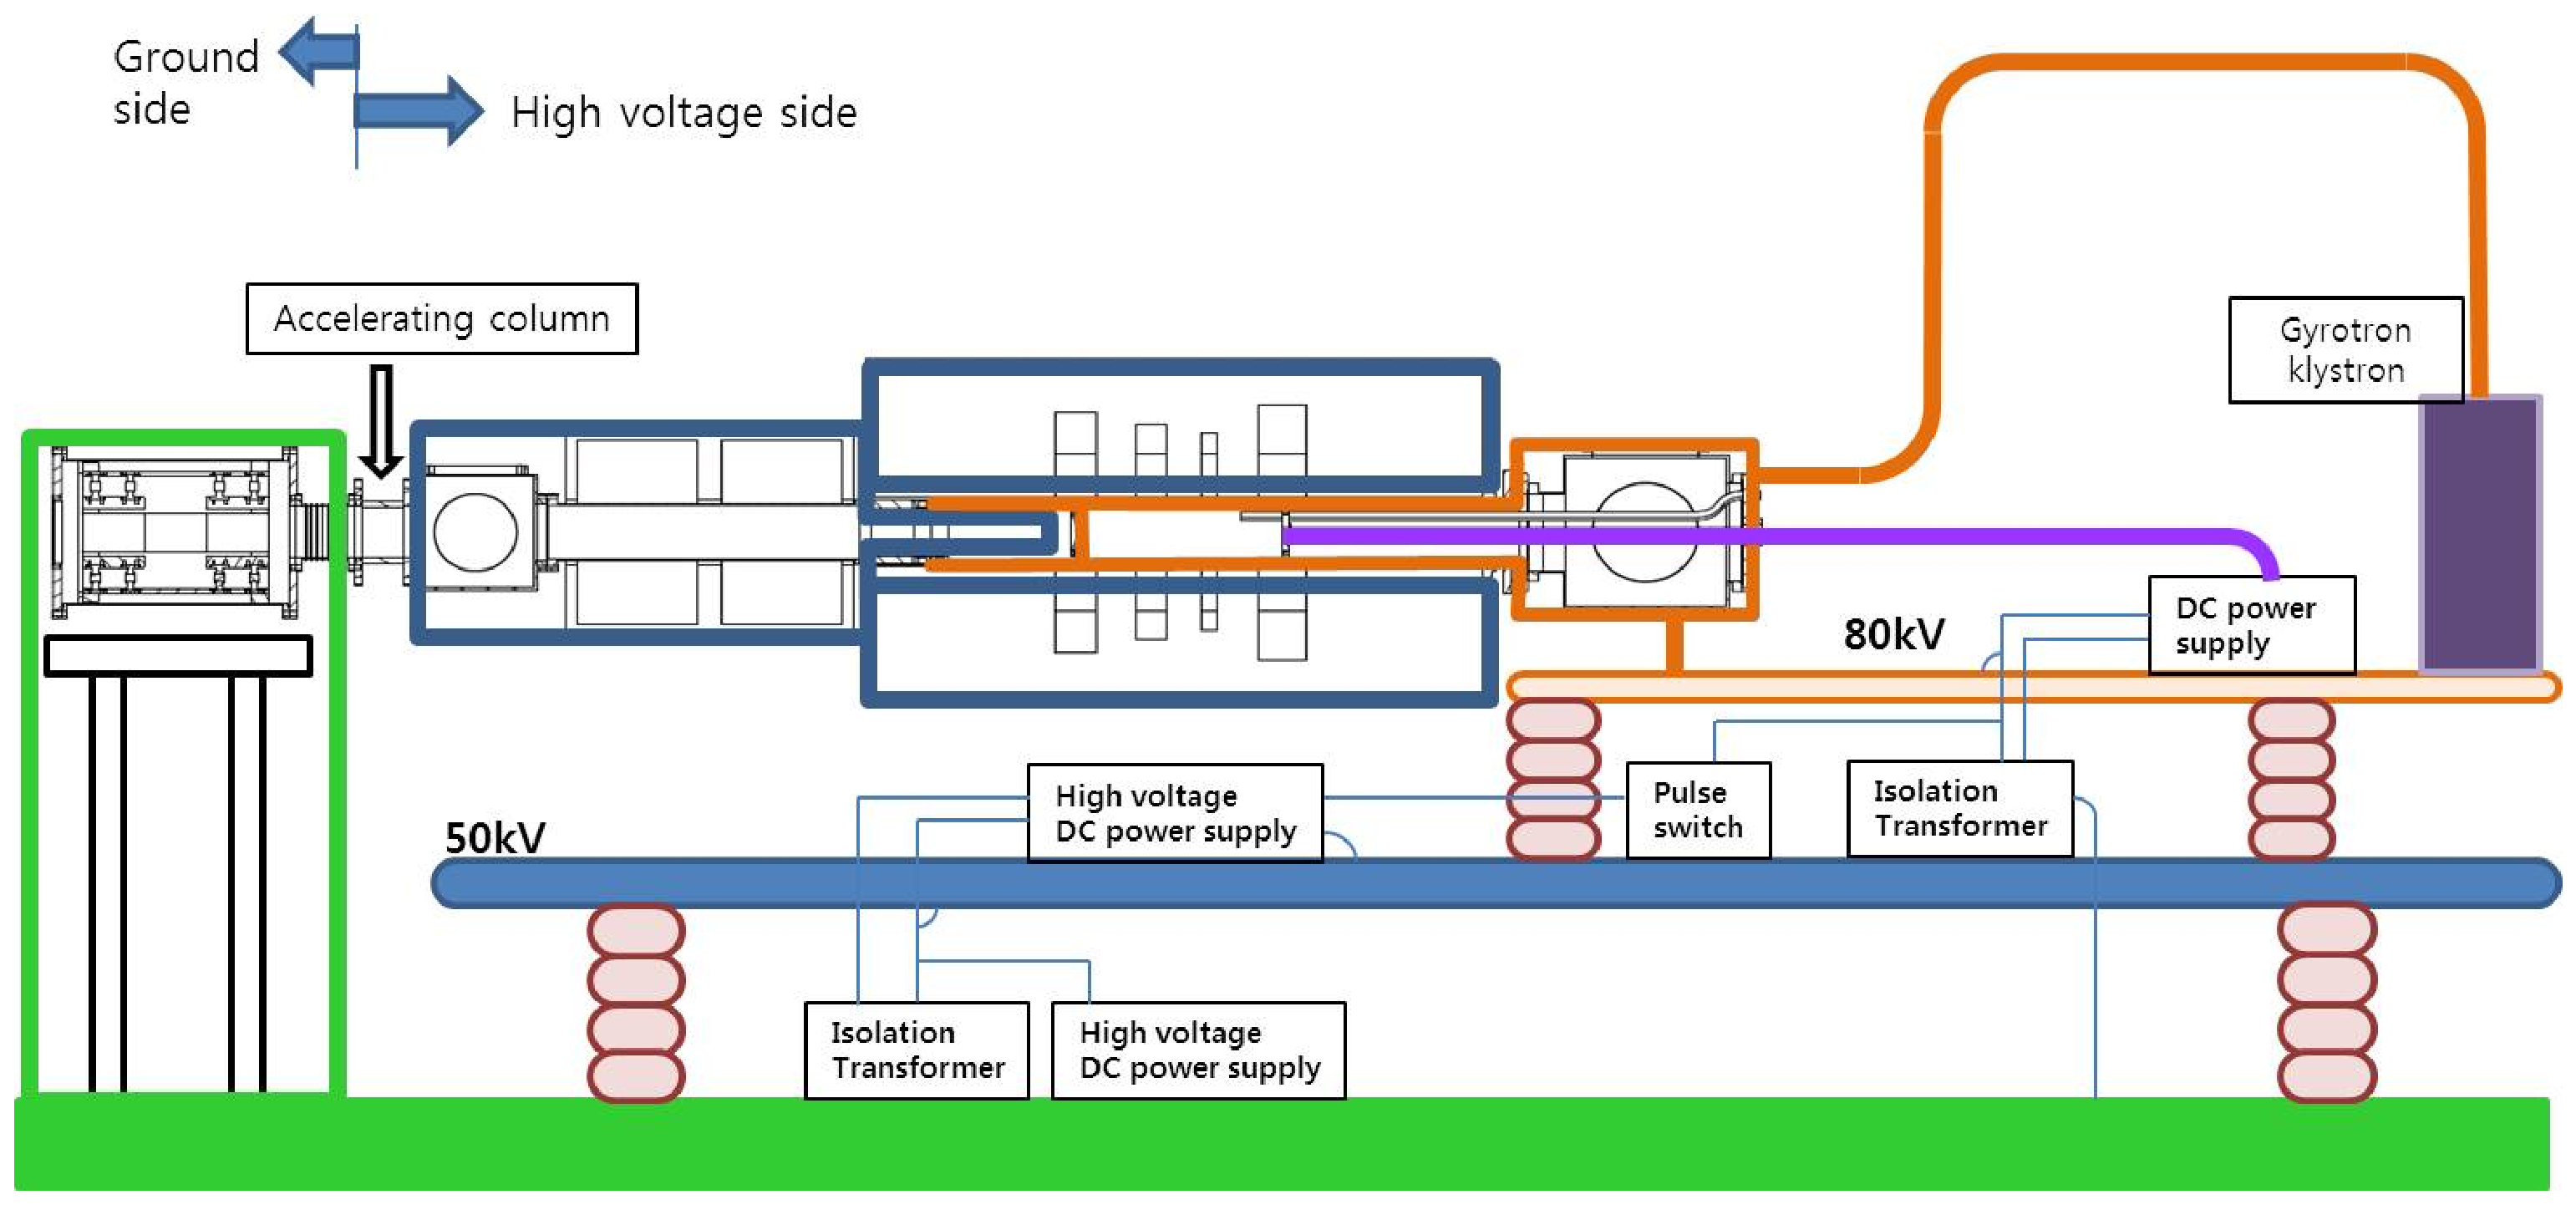
\includegraphics[width=1\columnwidth]{./images/high_voltage.eps}
\end{figure}
The driver linac injector of the RAON consists of a 28-GHz superconducting Electron Cyclotron Radiation (ECR) ion source, the LEBT (low energy beam transport), the 500-keV/u RFQ (radio-frequency quadrupole) and the MEBT (medium energy beam transport). For the ECR ion source, superconducting magnets and dual high power RF sources of 28 GHz and 18 GHz are used to improve its performance [1]. The high voltage ion sources could get from two different high voltage platforms (50kV and 80kV).

\section*{Requirements}
\begin{mdframed}[roundcorner=10pt]
\begin{itemize}
\item Connecting related equipment (Gauge Controller \& TMP controller etc.) \\ 
\item Development of AB PLC Ladder Program (Vacuum control \& Interlock)\\
\item Make Human-Machine Interface (HMI) program \\
\item Development the EPICS IOC \\
\item Serial communication for Gauge Controller \& TMP controller \\
\end{itemize}
\end{mdframed}


\section*{PLC control}
\begin{mdframed}[roundcorner=10pt]
\vspace{2mm}
\begin{figure}[H]
  \centering
  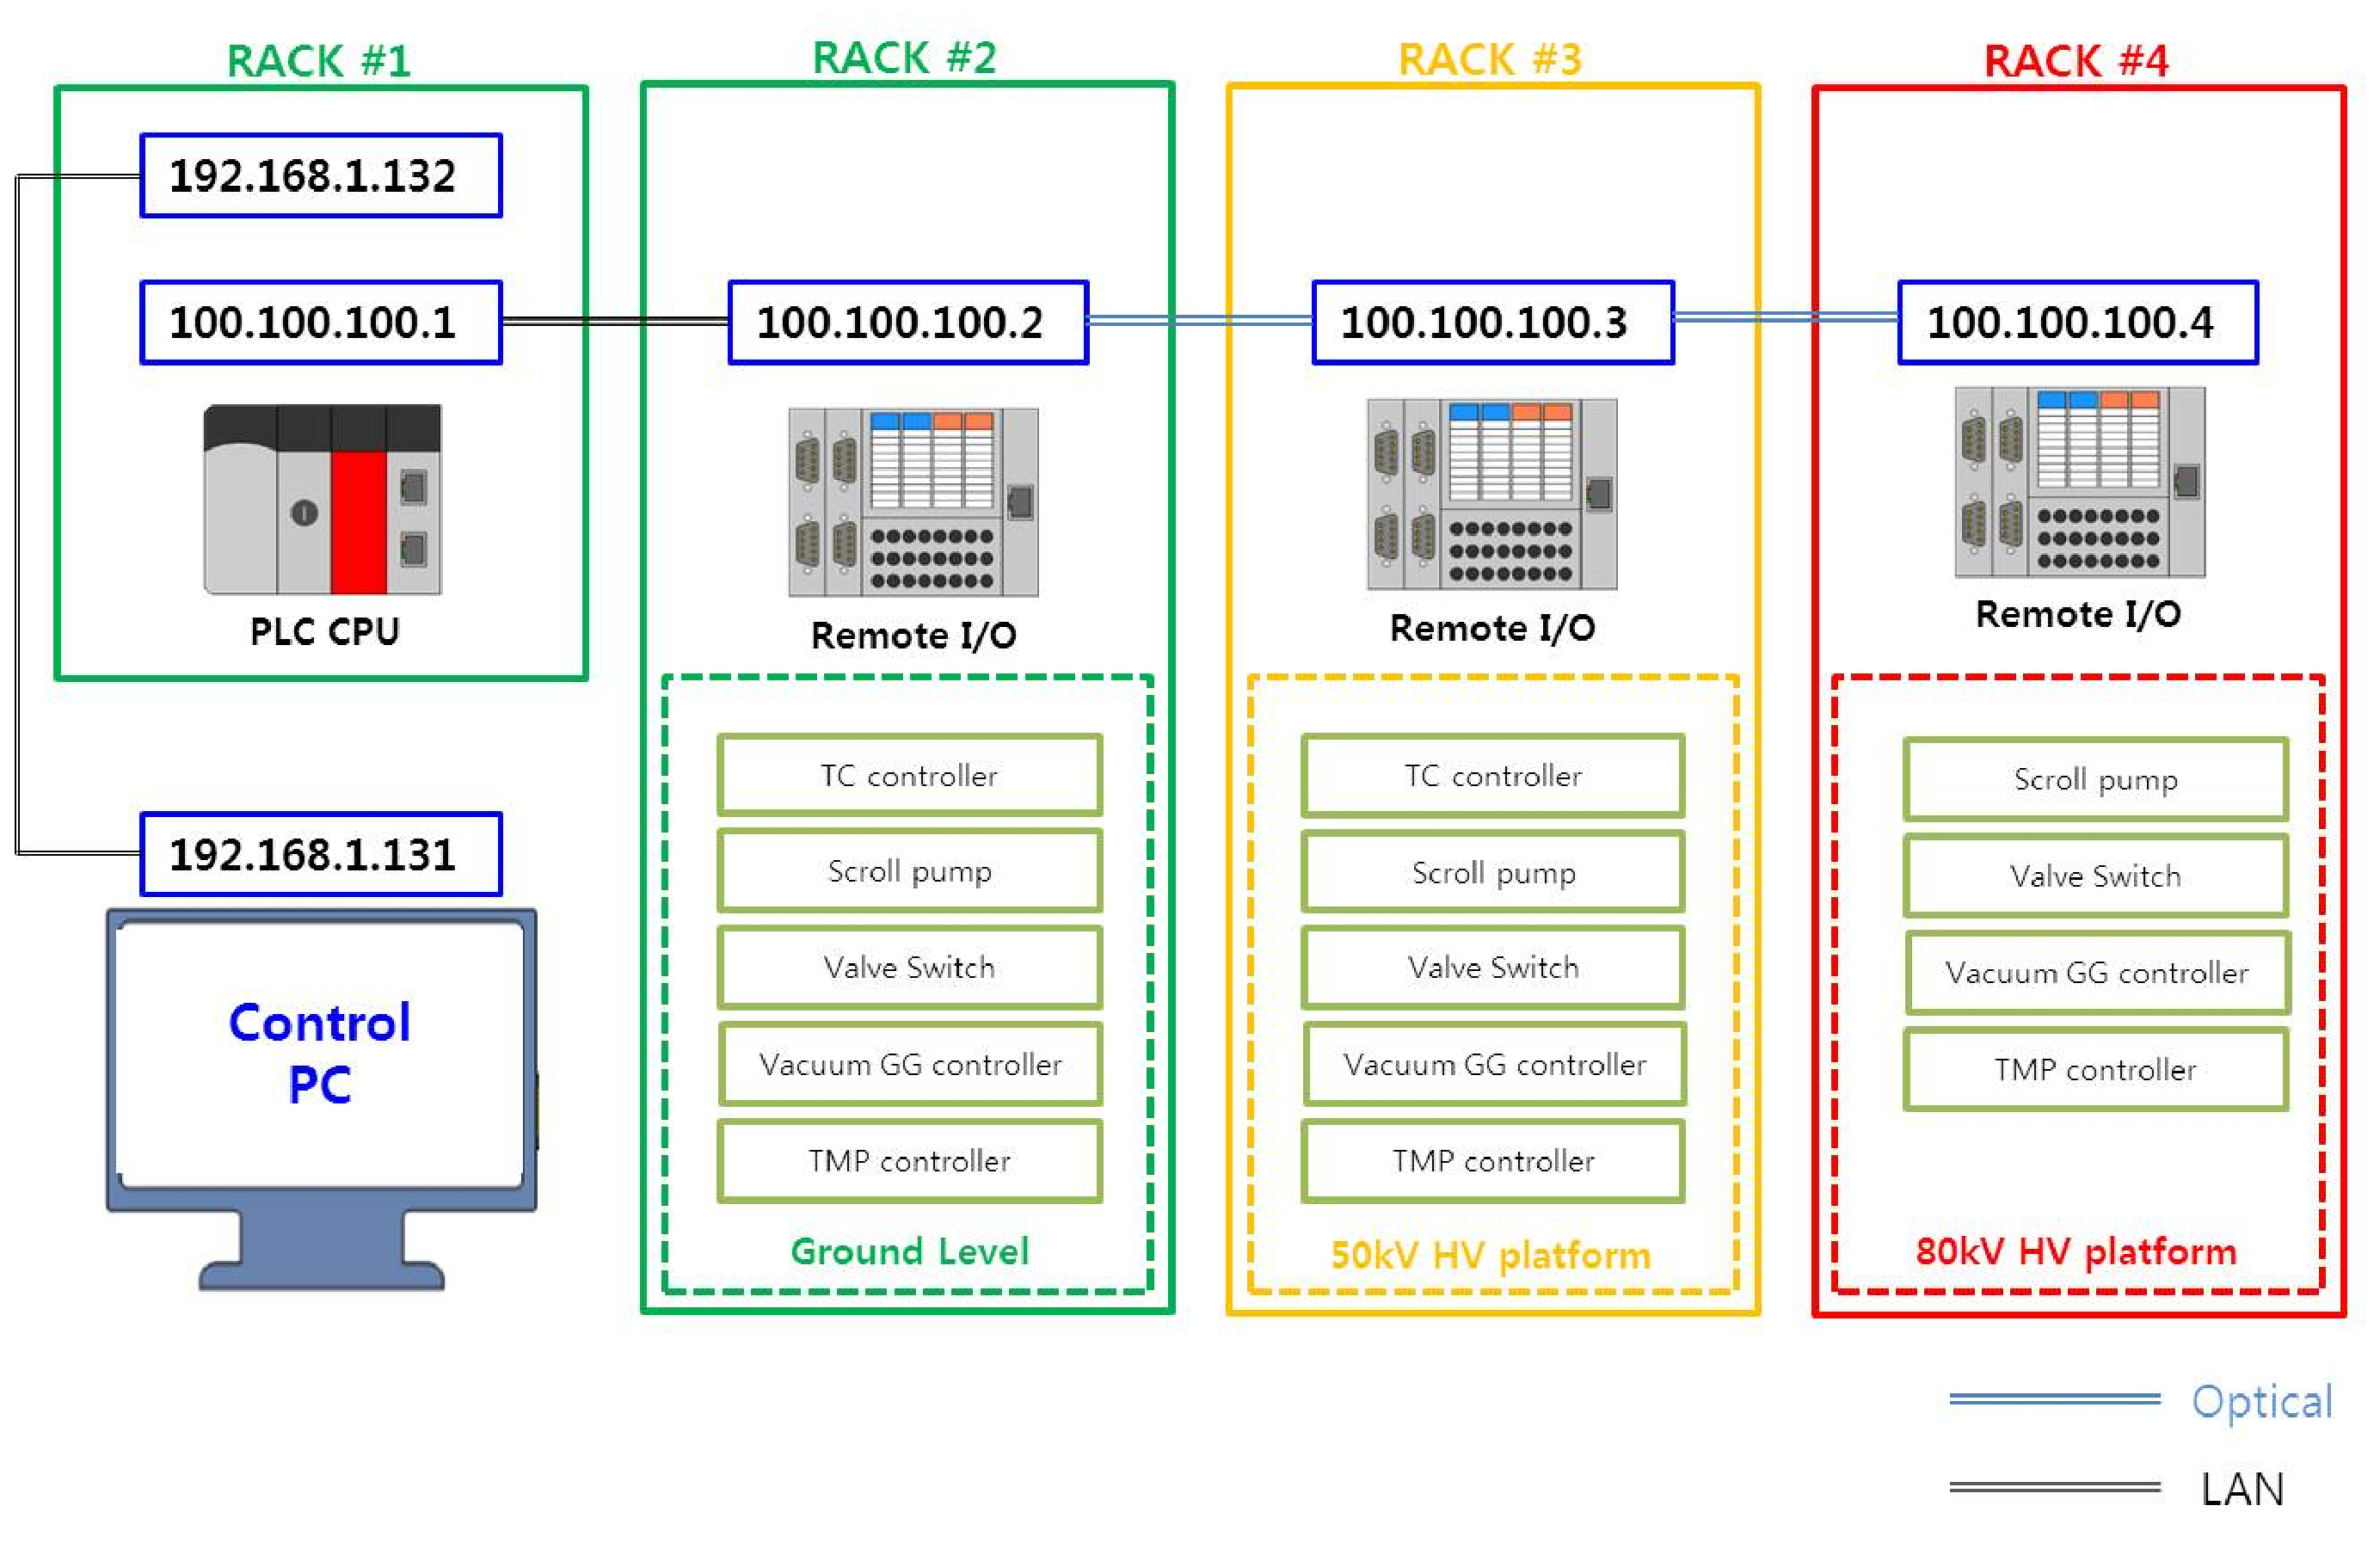
\includegraphics[width=1\columnwidth]{./images/vacuu_network_configuration.eps}
  %\caption{Overall architecture of the RAON control system}
  \label{fig:architecture}
\end{figure}

\begin{itemize}
\item Vacuum system of the ECR ion source is controlled by AB PLC \\
\item Interlock system performed with ladder logic program \\
\item There are used LAN \& optical cable to configure the network system \\
\end{itemize}
\end{mdframed}


\columnbreak



\subsection*{Prelimiary test for Networking \& Installation}
\begin{mdframed}[roundcorner=10pt]
\begin{figure}[H]
  \centering
  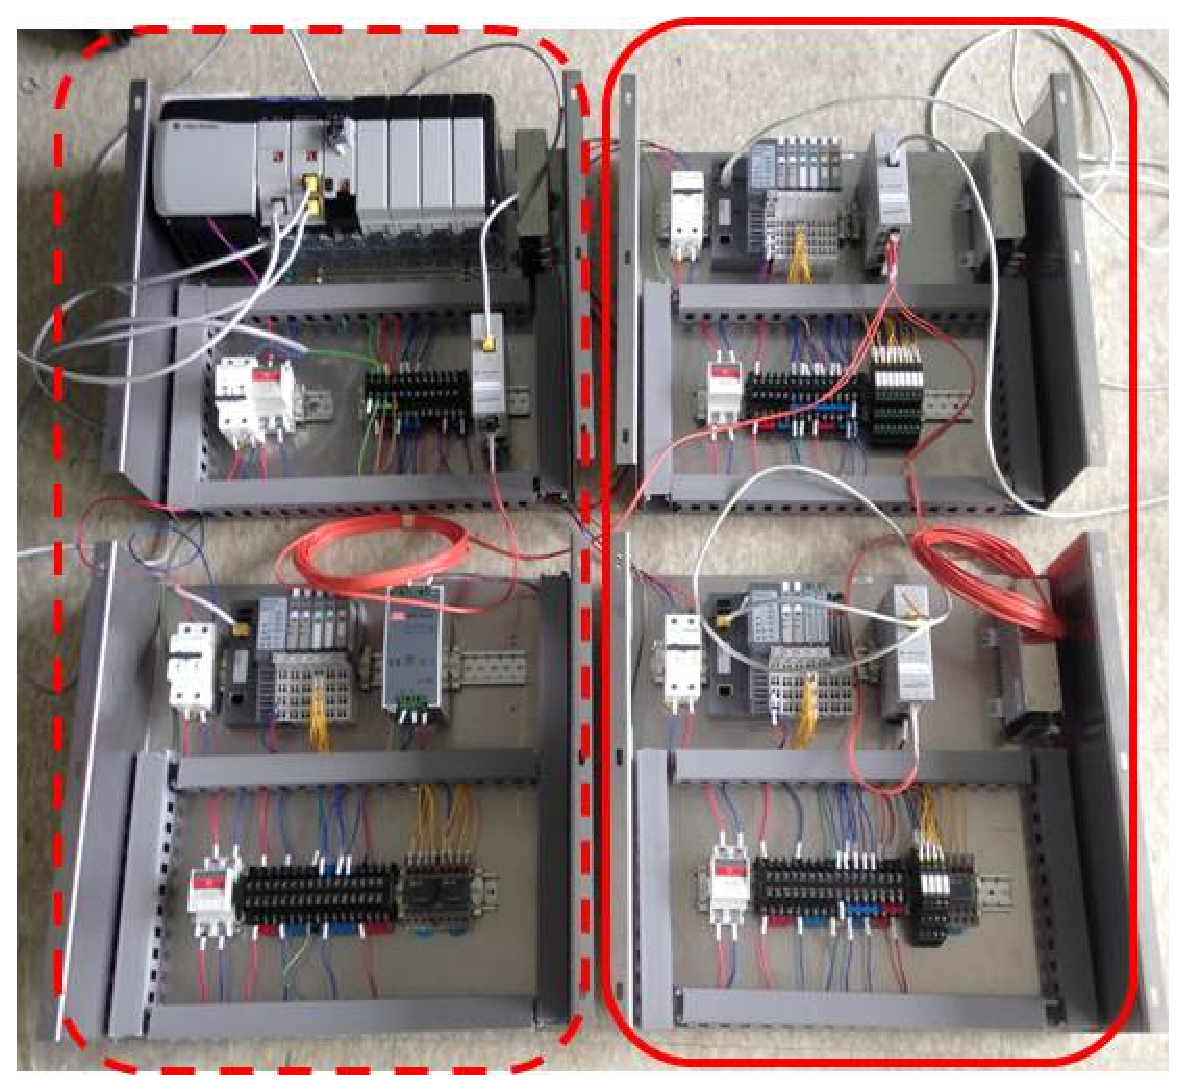
\includegraphics[width=1\columnwidth]{./images/Network_test.eps} \\
  \vspace{10mm}
\begin{itemize}
	\item Preliminary test set up for confirming teh network and I/O wiring. \\
\end{itemize}  
 \vspace{10mm}
  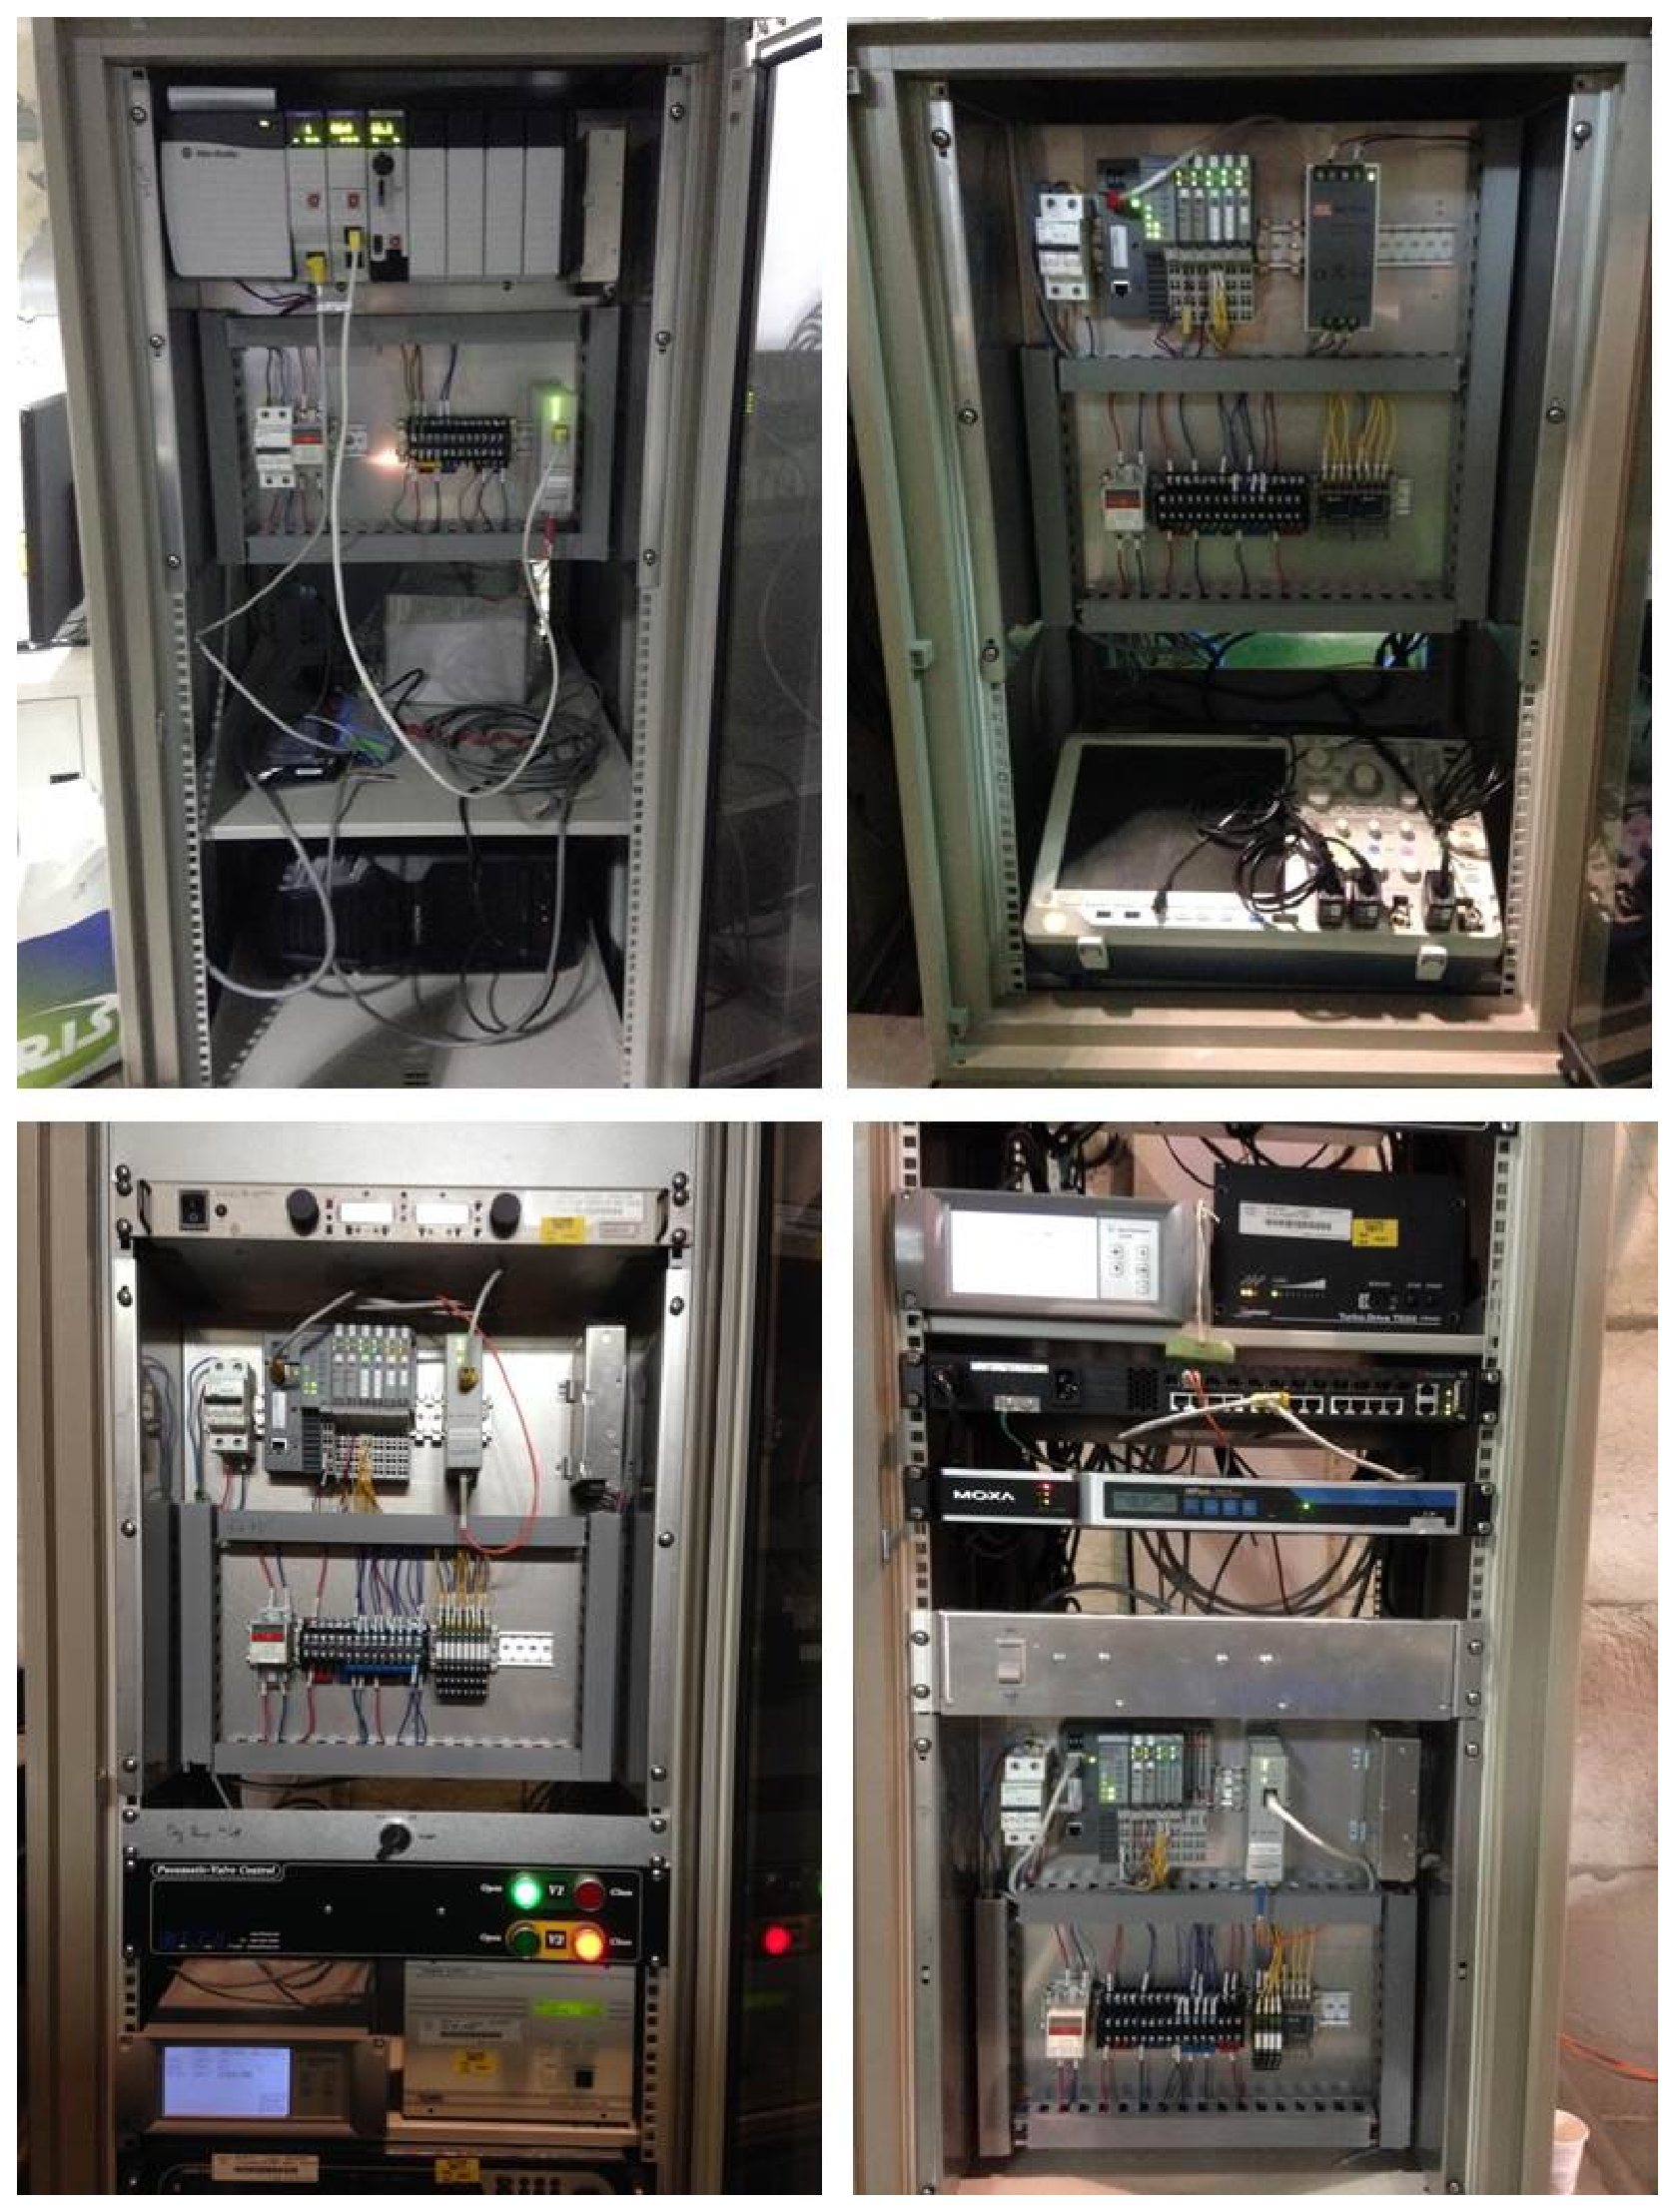
\includegraphics[width=1\columnwidth]{./images/install_total.eps} \\
  \vspace{10mm}
  \begin{itemize}
  	
  	\item PLC chassis installed at the each rack. 
  	\item OSAKA turbo pump controller (TD353) \& Vacuum gauge controller (XGS600) are connected with ASCII modules of AB PLC. 
  	\item Optical communication module (1734-ETAP2F) is installed to configure network system between ground platform and high voltage platform. 
  \vspace{10mm}
  \end{itemize}
  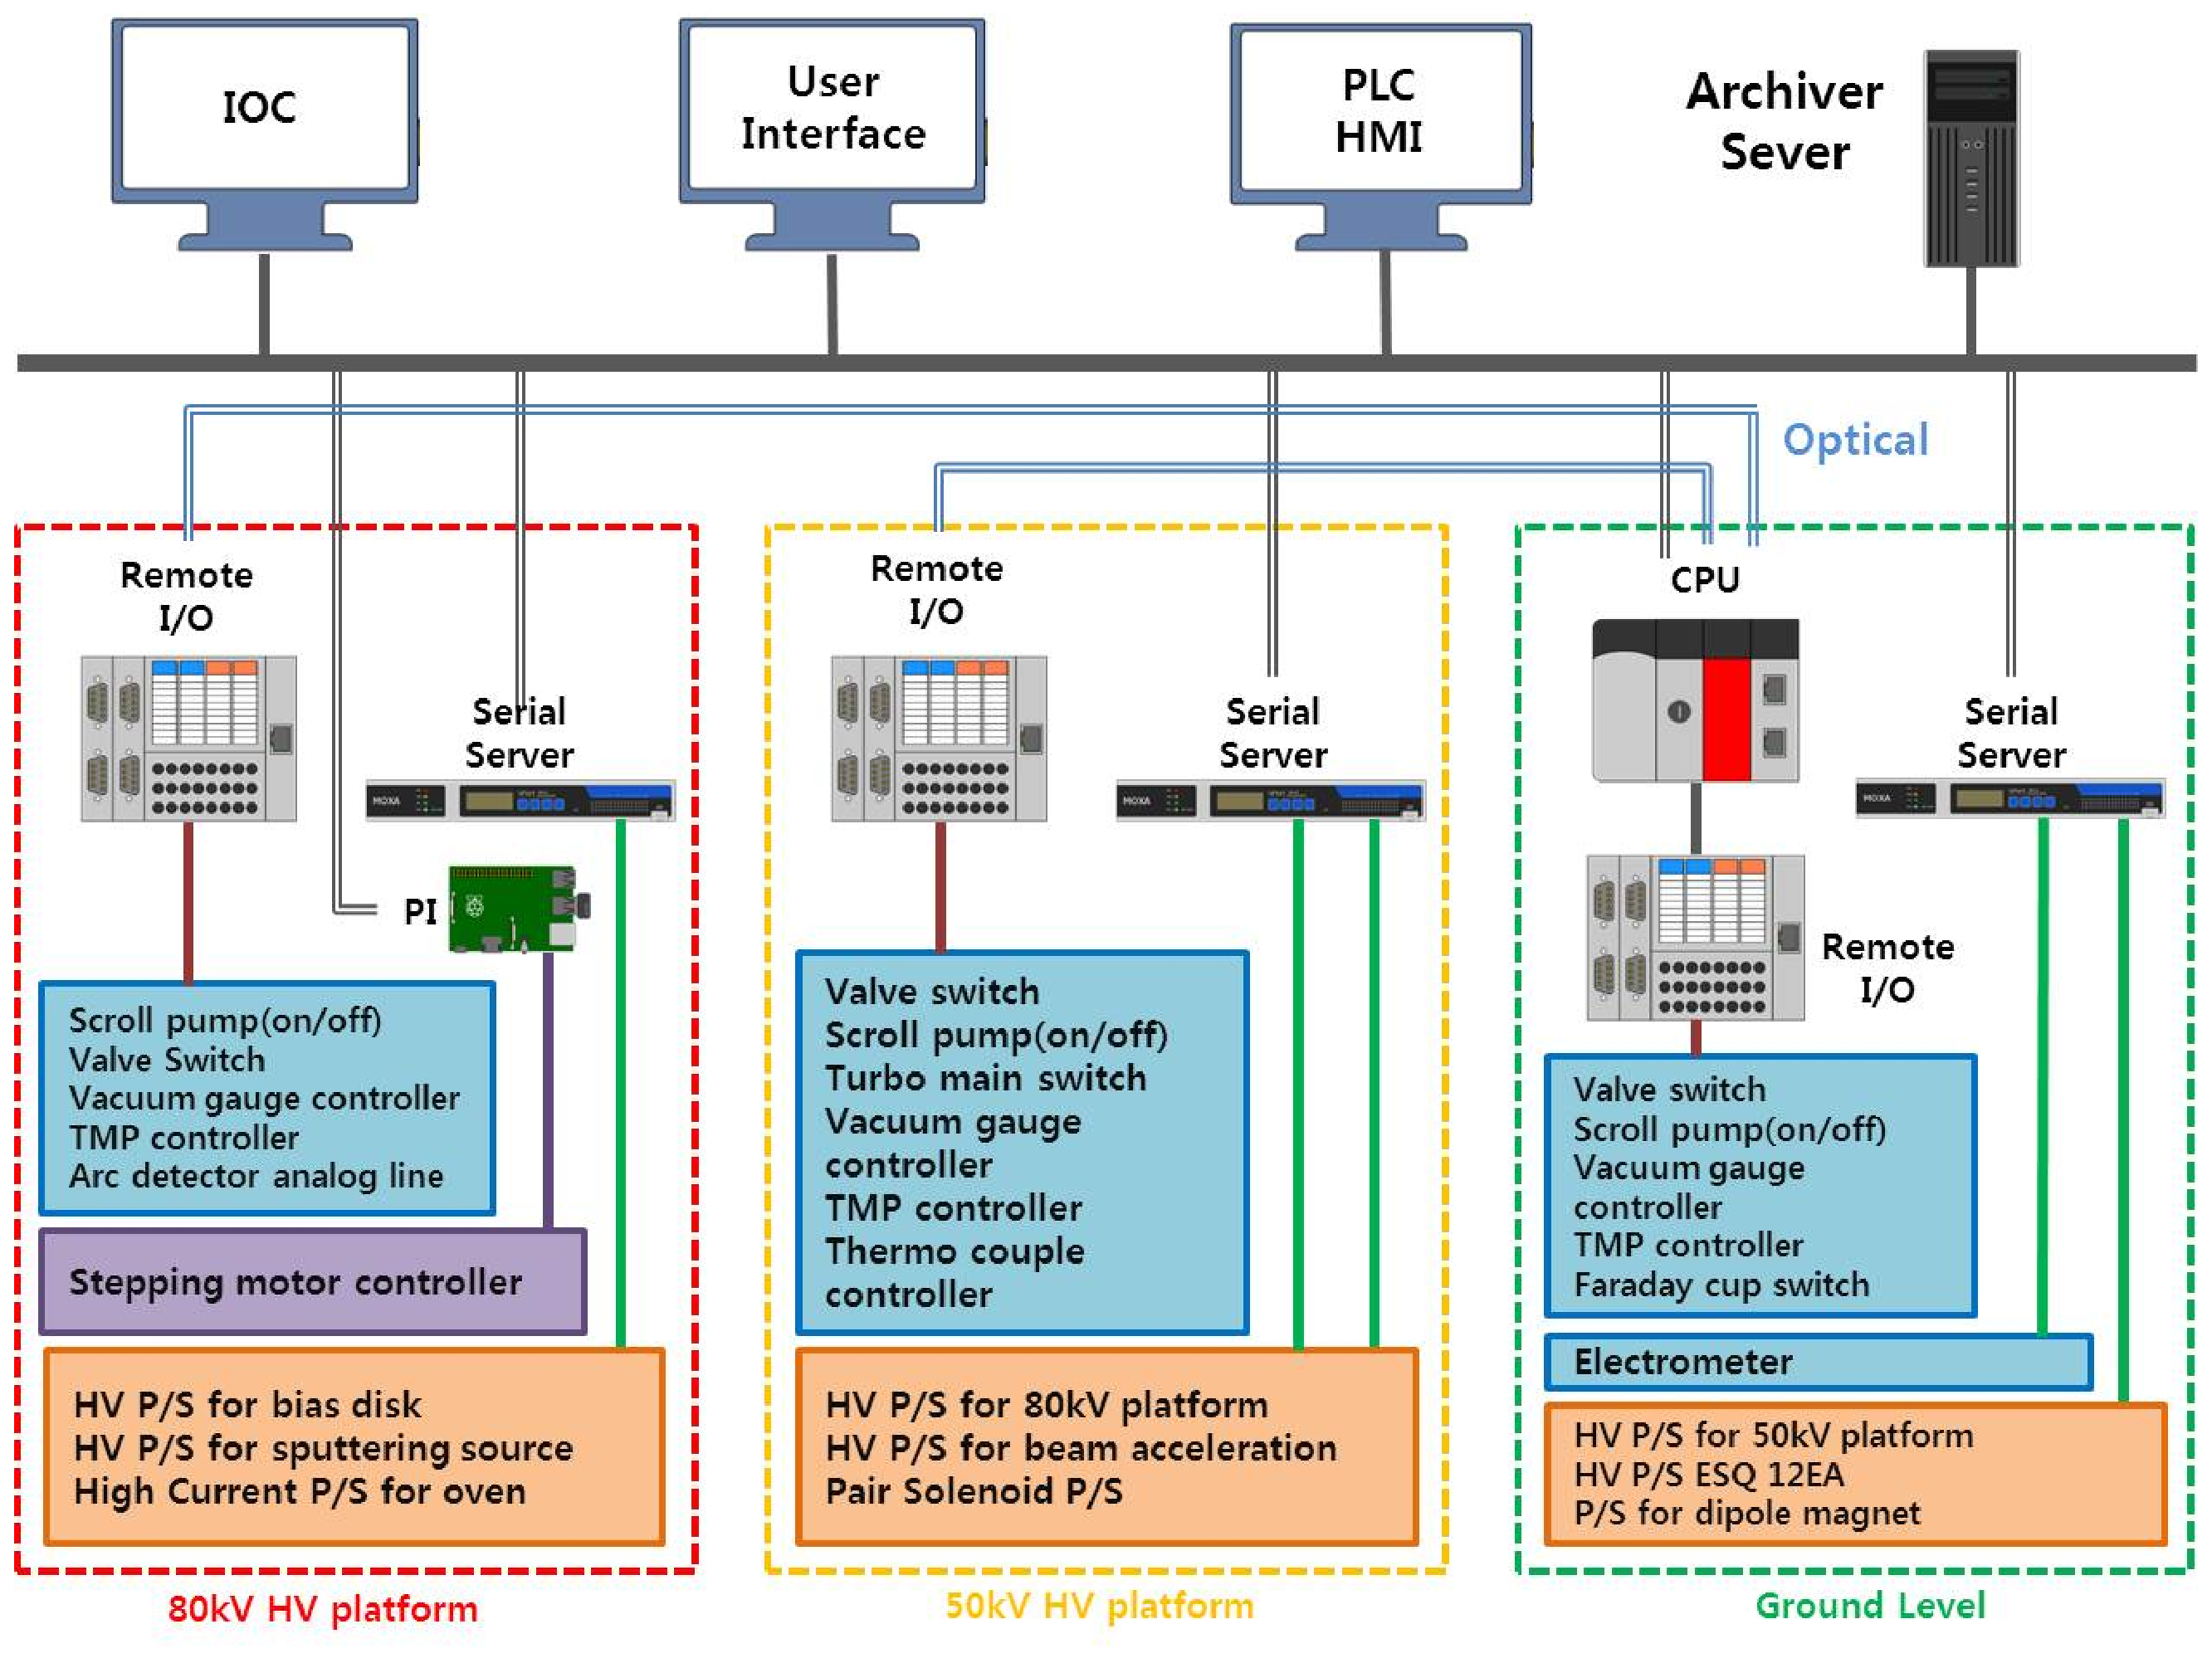
\includegraphics[width=1\columnwidth]{./images/control_system_ECR.eps} 
   
\end{figure}
\begin{itemize}
	\item The entire configuration of the ECR ion source vacuum system \\

\end{itemize}
\end{mdframed}


\columnbreak

% the EPICS IOC via Ethernet connection with time stamps given by EVR.
% In addition to the I/O board, a commercial/homemade FPGA board will be used for the signal processing.
% The PLC will be used for the front-end interface to the subsystems.
% The several vendors for PLC providing robust products, such as Allen-Bradley and SIEMENS, are considered.
% In addition the domestic PLC providers, such as LSIS~\cite{lsis}, are also considered in order to reduce the price.


%\begin{center}
%\rowcolors{1}{blue!20}{blue!6}
%\begin{tabularx}{0.934\columnwidth }{{ >{\hsize =0.30\hsize }X  >{\hsize =1.70\hsize }X}}
%\textbf{TDR}    & Technical Design Report \newline - build a testbed \\
%\textbf{LCS}    & Local Control System \newline  - build/test a prototype LCS for a dummy system\\
%\textbf{CCS I}  & Central Control System Part I\newline - design/test CCS from LCS and support subsystem prototypes\\
%\textbf{OPTIM}  & Optimization and Performance test \newline - check possible bottleneck for all connections\\
%\textbf{CCS II} & Central Control System  Part II \newline - setup the main control room\\
%\textbf{COMM}   & Commissioning \newline - maybe 24/7 works
%\end{tabularx}
%\end{center}


%\section*{Data management \& \\ System integration tool}



%Since XAL~\cite{XAL} has proved its usability and stability at Spallation Neutron Source (SNS) for several years,
%many recent accelerator projects such as CSNS, ESS, GANIL, TRIUMF, and FRIB, adopt
%this framework for building their own high level programming infrastructure.
%Moreover, the RAON control system demands the capabilities provided by XAL from the beginning of
%beam commissioning to the actual operation.
%Thus, the OpenXAL~\cite{OPENXAL}, an open source version of development framework,
%is selected as a high level application solution of the RAON control system.
%Using the object-oriented feature of Java,
%a hierarchical structure of the accelerator components will be modeled.
%Since there are many works to do, however, the international co-work is necessary.




\subsection*{Demo vacuum control system}

\begin{mdframed}[roundcorner=10pt]
\begin{figure}[H]
\centering
  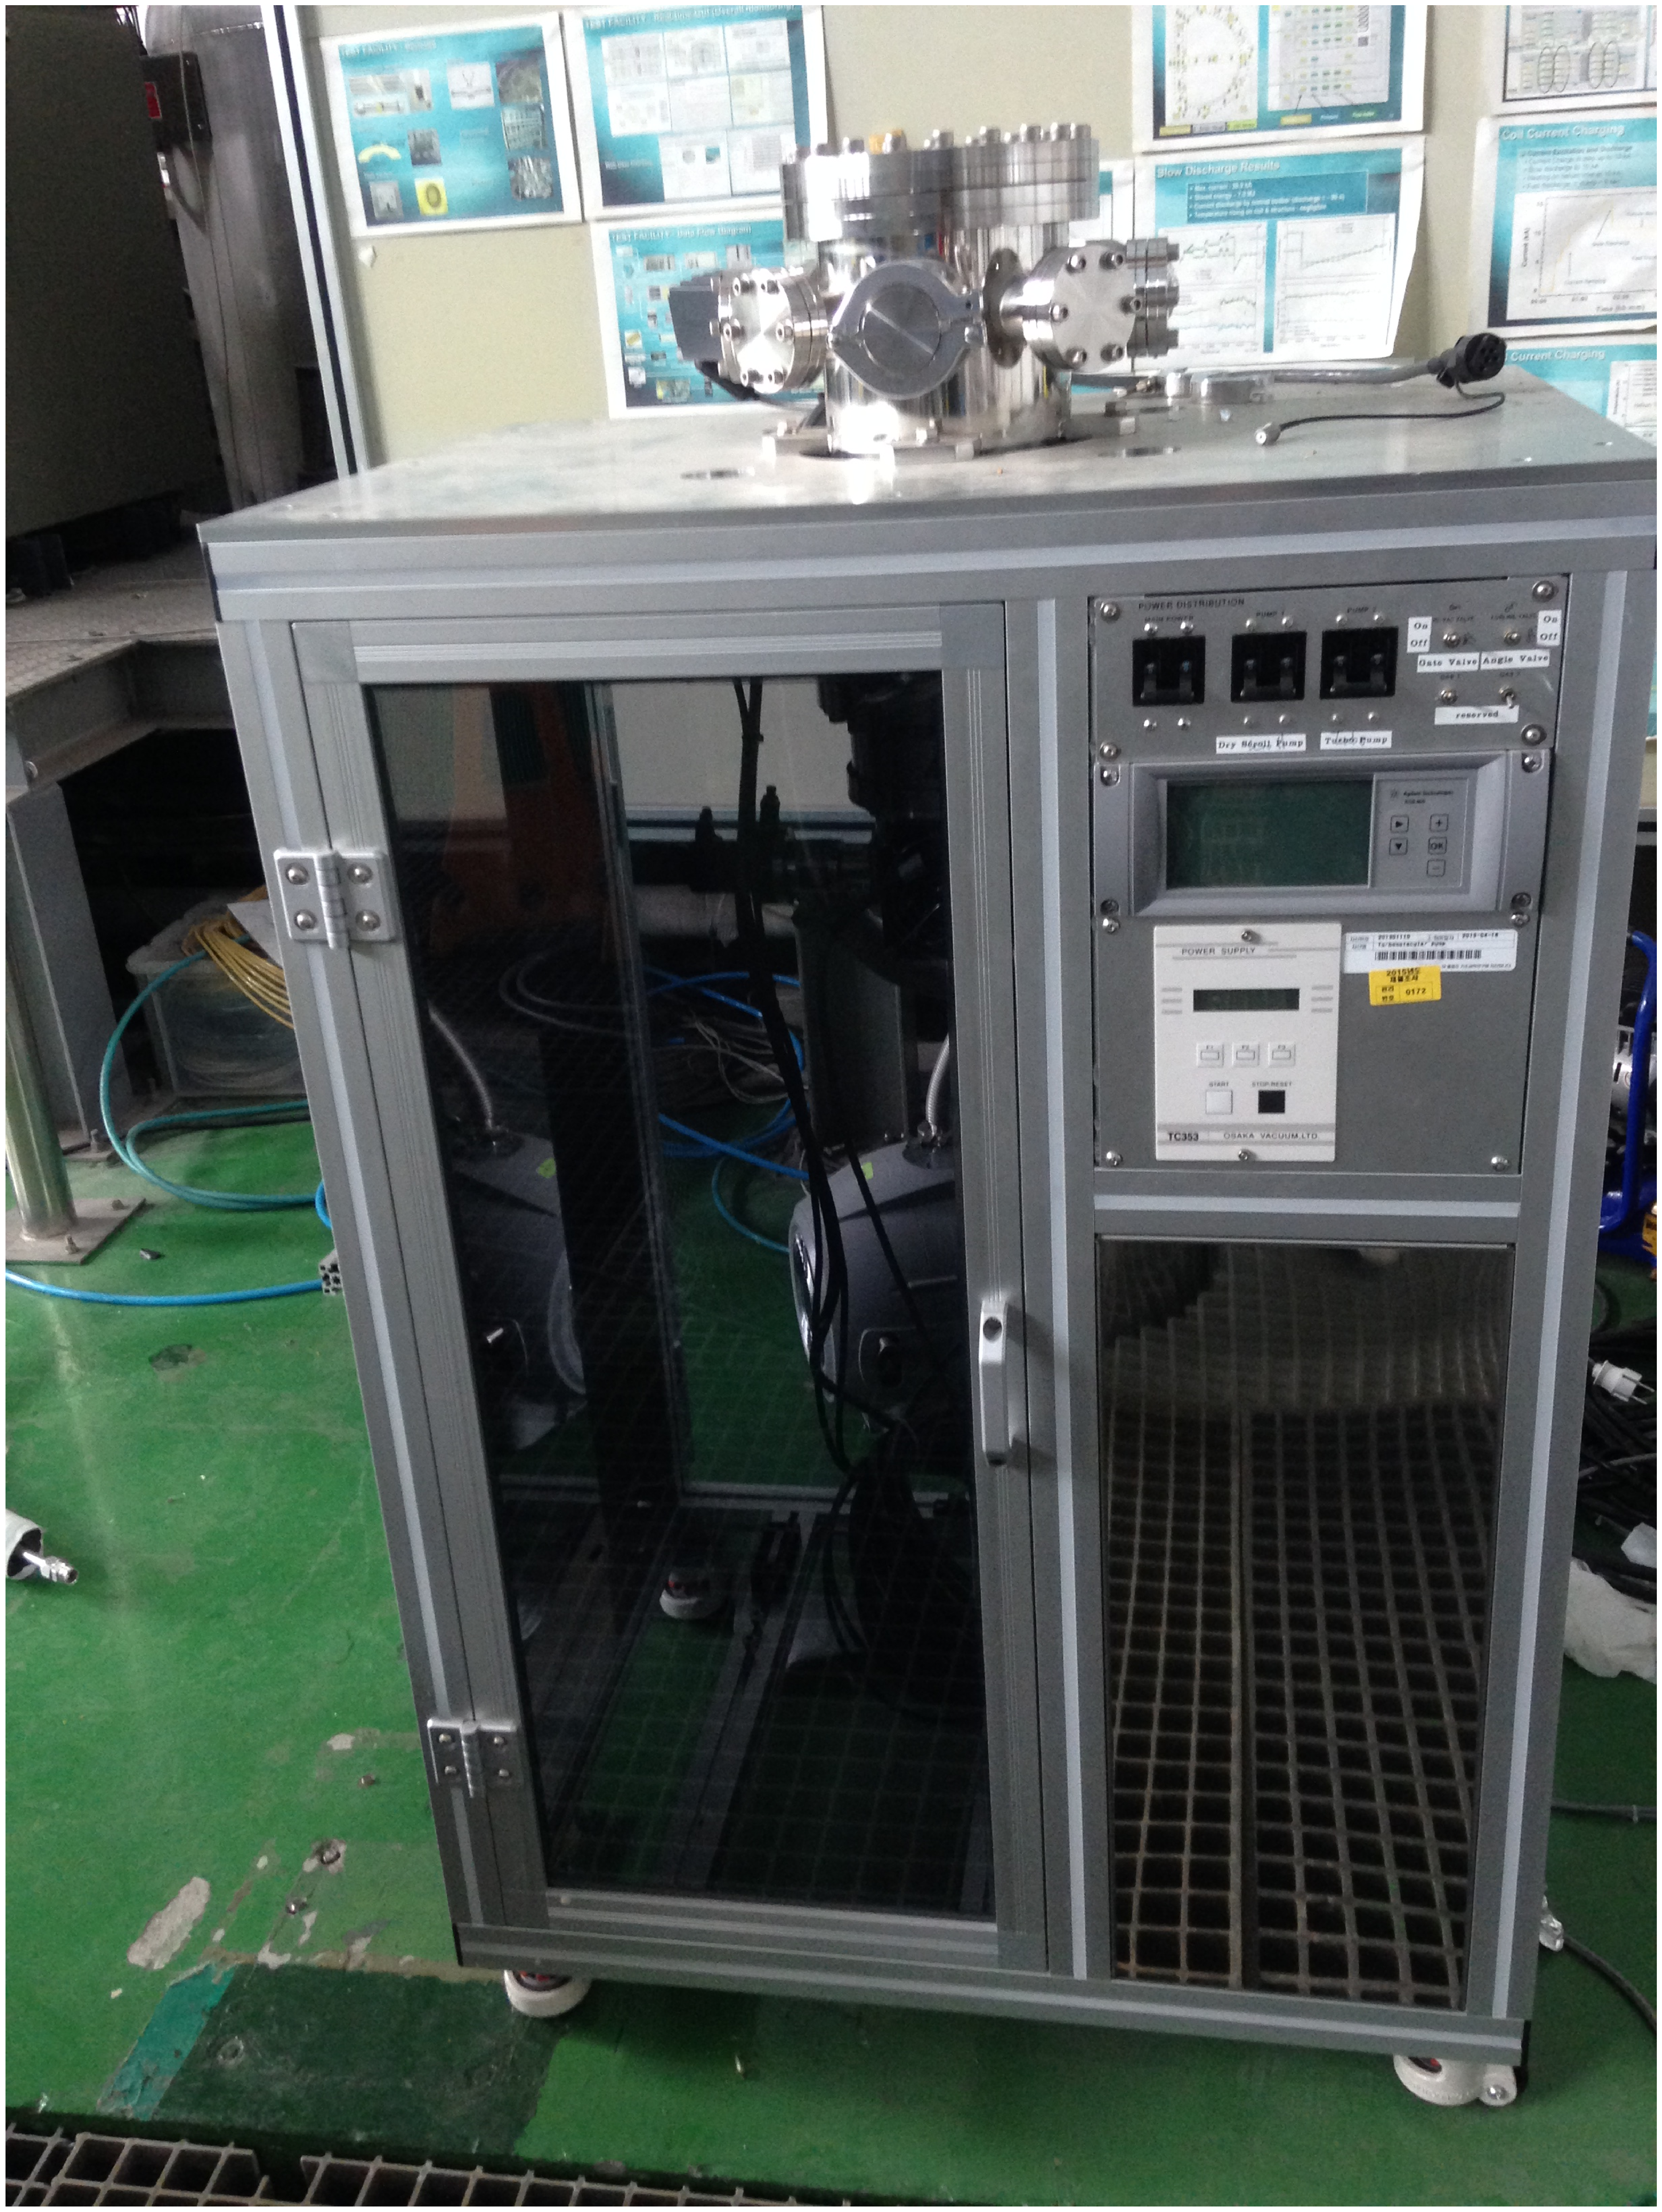
\includegraphics[width=1\columnwidth]{./images/vacuum_test.eps}
%\caption{The vacuum control system}
\label{fig:vacuum_control}
\end{figure}
\begin{itemize}
\item We configured demo vacuum control system like the vacuum system of the ECR ion source to test serial communication for turbo pump controller and vacuum gauge controller. 
\item The vacuum system controlled by PLC will be integrated with EPICS framework.
\end{itemize}
\end{mdframed}


\section*{Summary}
\begin{mdframed}[roundcorner=10pt]
The system will be integrated with EPICS framework through Modbus TCP/IP module or Ether-IP module of the AB PLC. We are developing the EPICS IOC to control the vacuum system in real-time using EPICS drivers. 
The User Interface (UI) for monitoring and operating the system will be developed by the Control System Studio (CSS) software to provide easy control environment for users.
The vacuum control system of the ECR ion source is finally designed by the ladder logic program to perform the interlock checks continuously without data from the EPICS IOC so that the PLC can perform its protection functions even when the IOC is  shut down [2].
\end{mdframed}

\section*{Acknowledgement}
This work is supported by the Rare Isotope Science Project funded by Ministry of Science, ICT and Future Planning(MISP) and National Research Foundation(NRF) of Korea(Project No. 2011-0032011).

\begin{thebibliography}{9}   % Use for  1-9  references
	%\begin{thebibliography}{99} % Use for 10-99 references
	
	\bibitem{Ref_1}
D. JEON et al., "Design of the RAON Accelerator System", Journal of the Korean Physical Society, Vol. 65, No. 7, October 2014,  pp. 1010 $\sim$1019.
	%\bibitem{TSHOO:NIMB} K.~Tshoo, {\it et. al},``Experimental systems overview of the Rare Isotope Science Project in Korea'',
	%Nucl. Inst. Meth. Phys. B. (2013)
	
	\bibitem{Ref_2}
M. E. Bannister?, F.W. Meyer, and J. Sinclair, ORNL, Oak Ridge, TN 37831-6372, USA
	
	
	%\bibitem{esstechnote0005}
	%G. Trahern, ``ESS Naming Convention'', ESS AD Technical Note.
	
	
\end{thebibliography}




\end{multicols}




%\vspace{13mm}

%\begin{minipage}[b]{1\linewidth}

%\section*{RAON Major Operations Modes}
%\vspace{2mm}
%\begin{figure}[H]
 % 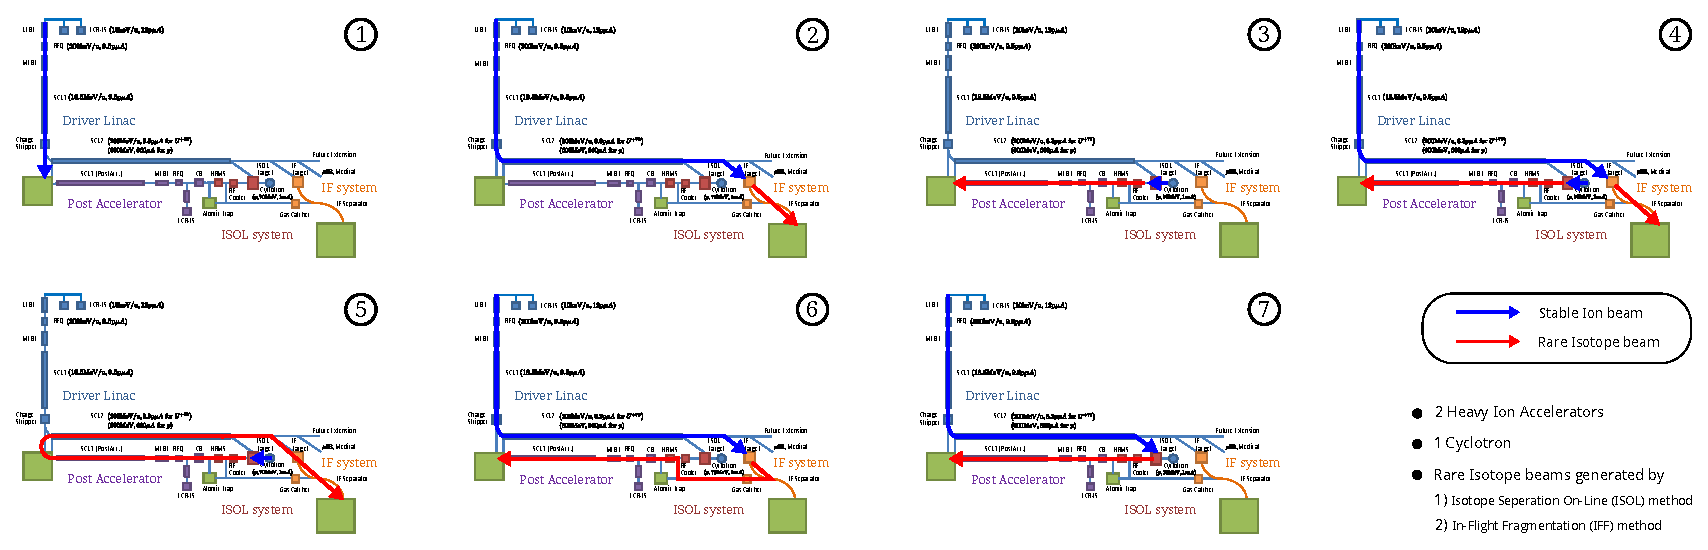
\includegraphics[width=0.99\columnwidth]{./images/raon_all_modes.eps}
%\end{figure}

%\end{minipage}





\end{document}

